\documentclass[addpoints]{exam}
\usepackage[T1]{fontenc}
\usepackage[utf8]{inputenc}

\usepackage[pdfencoding=auto, psdextra]{hyperref}
\usepackage{examfields}
\usepackage{totcount}
\usepackage{graphicx}
\usepackage{pdfcomment}
\usepackage{cleveref}

\pdfstringdefDisableCommands{\def\\{ }}
\def\DefaultOptionsofRadio{print,notoggletooff,radiosymbol=\ding{108}}

\regtotcounter{section}

\pagestyle{headandfoot}
\header{CSC XXX}{}{Demo Assessment, 2021}
\footer{}{Page \thepage\ of \numpages.}{}

\begin{document}

\begin{coverpages}
  \begin{center}
    \large
    UNIVERSITY OF TORONTO\\
    Faculty of Arts and Science\\[.5cm]

    DEMO FINAL ASSESSMENT 2021\\[.5cm]

    CSC XXX\\[.5cm]

    Duration - as long as you'd like; probably 2 minutes. \\[.5cm]

    This assessment does not count towards your final grade and is entirely
    optional. It is intended to ensure your PDF viewer meets the technical
    requirements necessary to complete your upcoming assessment. \\[.5cm]

    Feel free to ask your friends for help. Whatever.
  \end{center}

  \hrule\vspace*{1em}
  \begin{minipage}{0.9\textwidth}
    \FullTextField[name=name]{Name: } \\
    \\ \FullTextField[name=studentno,maxlen=10]{Student Number: } \\ \\
    \\
      % \begin{minipage}{\textwidth}
    \noindent Rules:
    \begin{enumerate}
    \item Make sure to fill in your name and student number in the fields.
    \item You must also acknowledge your commitment to academic integrity
          after completing this assessment by checking the box below.
    % sdrobert: why are these under "Rules"
    % \item This exam paper contains \numpages\ pages.
    % \item There are \total{section}\ sections in this exam.
    % \item There are \numquestions\ questions in this exam, worth a total of
    %       \numpoints\ marks.
    \end{enumerate}

    \textbf{ %
      Failure to comply with the above rules will result in an automatic
      grade of zero.
    }

    \begin{center}
      \fbox{\fbox{\parbox{5.5in}{\centering\vspace*{.5em}
        \begin{minipage}{0.9\textwidth}
        \emph{%
          By checking the following box, I confirm that my conduct during this
          assessment adheres to the
          \href{https://governingcouncil.utoronto.ca/secretariat/policies/code-behaviour-academic-matters-july-1-2019}{Code of Behaviour on Academic Matters}.
          I confirm that I did not act in such a way that would constitute cheating,
          misrepresentation, or unfairness, including but not limited to, using
          unauthorized aids and assistance, personating another person, and
          committing plagiarism.
          %
        }

        \hfill\CheckBox[name=integrity]{\textbf{Check here:}}
        \end{minipage}
        \vspace*{.5em}
      }}}
    \end{center}
  \end{minipage}
  \vspace*{1em}\hrule

  \begin{center}
    \pointtable[v][questions]
  \end{center}
\end{coverpages}

\begin{Form}
\begin{questions}

  \section{English} %%%%%%%%%%%%%%%%%%%%%%%%%%%%%%%%%%%%%%%%%%%%%%%%%%%%%%

  \question[1]
  \MultipleChoice[name=randj]{
    In Shakespeare's famous tragedy of 1597 \textit{Romeo \& Juliet},
    Romeo \& Juliet:
  }{%
    guns={were discovered by Baz Luhrmann to have used guns, not swords.},%
    smell={introduced \textit{Smell-O-Vision} to theatre performances.},%
    characters={are characters in the play.}%
  }

  \question[3]
  \FullTextField[multiline,name=poem,below]{%
    Write a poem. It must be at least three lines to receive full marks.
  }

  % English %%%%%%%%%%%%%%%%%%%%%%%%%%%%%%%%%%%%%%%%%%%%%%%%%%%%%%%%%%%%%%

  \newpage
  \section{Mathematics} %%%%%%%%%%%%%%%%%%%%%%%%%%%%%%%%%%%%%%%%%%%%%%%%%%

  \question \label{ques:math}
  \begin{parts}
    \part[1] \label{part:nat}
    \NumericField[integer, low=1, high=10, name=chosennum]{%
      Pick a natural number from 1 to 10:}

    \part[1]
    \MultipleChoice[name=isfive]{Was it 5?}{Yes,No}

    \part[4]
    \MultipleAnswer{Select all that are 5}{%
      firstfive={5},%
      secondfive={5},%
      notfive={6},%
      thirdfive={5}%
    }

  \end{parts}

  % Mathematics %%%%%%%%%%%%%%%%%%%%%%%%%%%%%%%%%%%%%%%%%%%%%%%%%%%%%%%%%%

  \newpage
  \section{Fine Art} %%%%%%%%%%%%%%%%%%%%%%%%%%%%%%%%%%%%%%%%%%%%%%%%%%%%%

  \begin{center}
    \pdftooltip{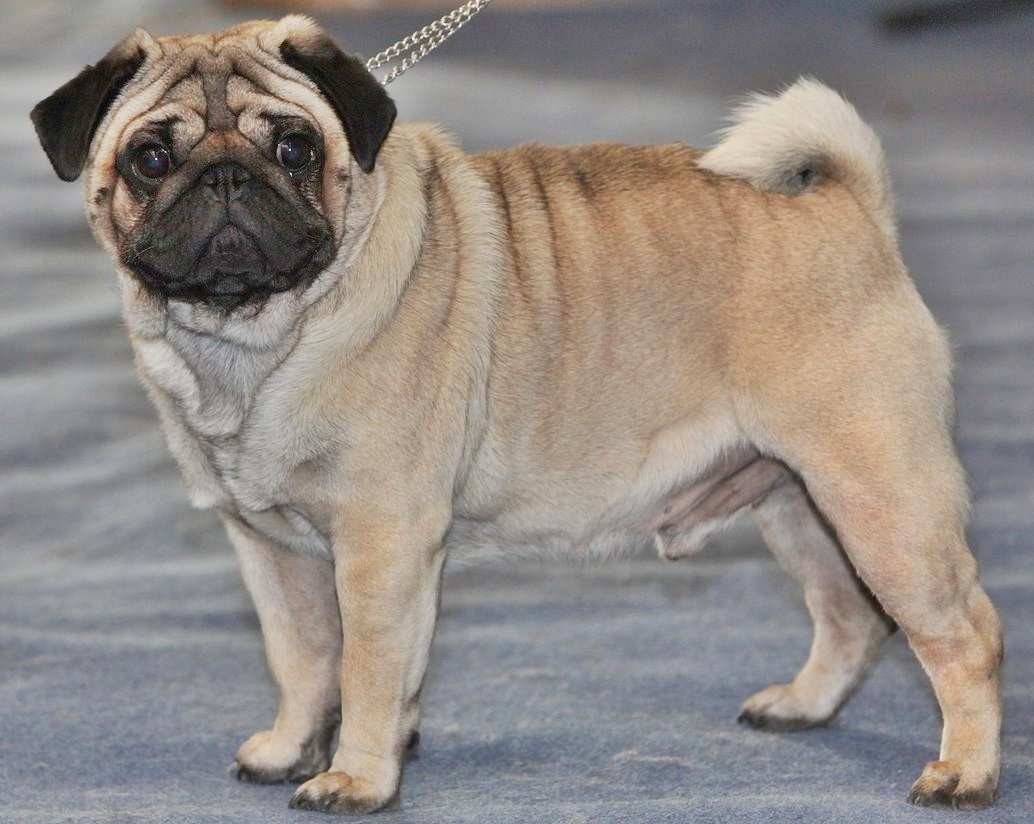
\includegraphics[width=.5\textwidth]{pug.jpg}}{A pug, Mops}
    \url{https://www.flickr.com/photos/dalli/3982174152/}
  \end{center}

  \question[1]
  \MultipleChoice[name=pug]{What does this picture represent?}{%
    sausage={A sausage.},%
    dog={A dog.},%
    antoinette={Marie Antoinette.}%
  }

  % Fine Art %%%%%%%%%%%%%%%%%%%%%%%%%%%%%%%%%%%%%%%%%%%%%%%%%%%%%%%%%%%%%

\end{questions}
\end{Form}

\cfoot{Page \thepage\ of \numpages. End of assessment.}
\end{document}